\documentclass[12pt]{article}

\usepackage[margin=1in]{geometry}
\usepackage{amsmath}
\usepackage{amsfonts}
\usepackage{amssymb}
\usepackage{graphicx}
\usepackage{booktabs}
\usepackage{float}
\usepackage{hyperref}
\usepackage{cite}
\usepackage{rotating}
\usepackage{subcaption}

\newcommand{\E}{\mathbb{E}}
\newcommand{\Var}{\mathbb{V}}

\title{MGTECON 603 - Problem Set 4\\ \small{(Instructor: Guido Imbens)}}
\author{Wooyong Park\\ {\small Collaborators: Cem Kozanoglu, Roberto Gonzalez Tellez, Hanniel Ho, Aileen Wu}}
\date{\today}

\begin{document}

\maketitle

\section*{0 Summary Statistics}

The summary statistics of the data are shown in table \ref{tab:summary_stats} in the appendix.

Also, the scatterplot and the correlation matrix of the data are shown in figure \ref{fig:scatterplot_matrix} in the appendix.



\section{Problem 1}

\subsection{Construct Age and Wage Variables}

I constructed the age variable as age = 1990 - year of birth and the wage variable as wage = exp(log wage).

\subsection{Summary Statistics}

Based on the results from the R script:

\begin{itemize}
    \item Mean age: 1955.397 years (standard deviation: 2.905 years)\footnote{The age variable is constructed as age = 1990 - \texttt{yob} in the .txt format dataset. If you consider the \texttt{yob} variable to have omitted 1900 in front, then the mean age is 1955.397 - 1900 = 55.397 years.}
    \item Mean wage: \$439.47 (standard deviation: \$364.94)
\end{itemize}

The age distribution appears to be concentrated around the mean, indicating a relatively homogeneous sample in terms of birth year. The wage distribution shows substantial variation with a standard deviation nearly as large as the mean, suggesting significant income inequality in the sample.

\section{Problem 2}

\subsection{OLS Regression Results}

I estimated the following regression model:
$$wage_i = \beta_0 + \beta_1 \cdot educ_i + \varepsilon_i$$

The regression results show:


\begin{table}[h]
\begin{center}
\begin{tabular}{l c c}
\hline
 & Homoskedastic & White-Robust \\
\hline
(Intercept)             & $61.1954^{***}$ & $61.1954^{***}$ \\
                        & $(2.4623)$      & $(2.5964)$      \\
educ                    & $29.6224^{***}$ & $29.6224^{***}$ \\
                        & $(0.1868)$      & $(0.2102)$      \\
\hline
Num. obs.               & $329509$        & $329509$        \\
R$^2$ (full model)      & $0.0709$        & $0.0709$        \\
% R$^2$ (proj model)      & $$              & $$              \\
Adj. R$^2$ (full model) & $0.0709$        & $0.0709$        \\
% Adj. R$^2$ (proj model) & $$              & $$              \\
\hline
\multicolumn{3}{l}{\scriptsize{\begin{minipage}{0.9\linewidth}\scriptsize\textit{Notes:} 
  The table shows two regression models: one with homoskedastic standard errors 
  and one with Eicker–Huber–White robust standard errors.\end{minipage}}}
\end{tabular}
\caption{Regression of wage on years of education}
\label{tab:problem_2_model}
\end{center}
\end{table}


The education coefficient is highly significant ($p < 0.001$). Each additional year of education is associated with approximately \$29.62 higher wages on average.

\subsection{Homoskedasticity vs. Heteroskedasticity}

The comparison between homoskedastic and heteroskedastic-robust standard errors reveals:

\begin{itemize}
    \item The homoskedastic standard errors are slightly smaller than the heteroskedastic-robust ones
    \item The heteroskedastic-robust standard error for the education coefficient increases from 0.1868 to 0.2102
\end{itemize}

\section{Problem 3}

\subsection{Residual Analysis}

To investigate the presence of heteroskedasticity, I computed the residuals and the squared residuals from the OLS regression and analyzed their relationship with years of education.
Since it is difficult to list these values for all observations in this document, I attached the scatter plots of the residuals and the squared residuals against the years of education in figure \ref{fig:residual_analysis} in the appendix.

\subsection{Average Squared Residuals by Education Level}

Figure \ref{fig:avg_squared_residuals_vs_educ} shows the average squared residuals versus years of education, which displays a clear upward trend, indicating heteroskedasticity.

\begin{figure}[h]
    \centering
    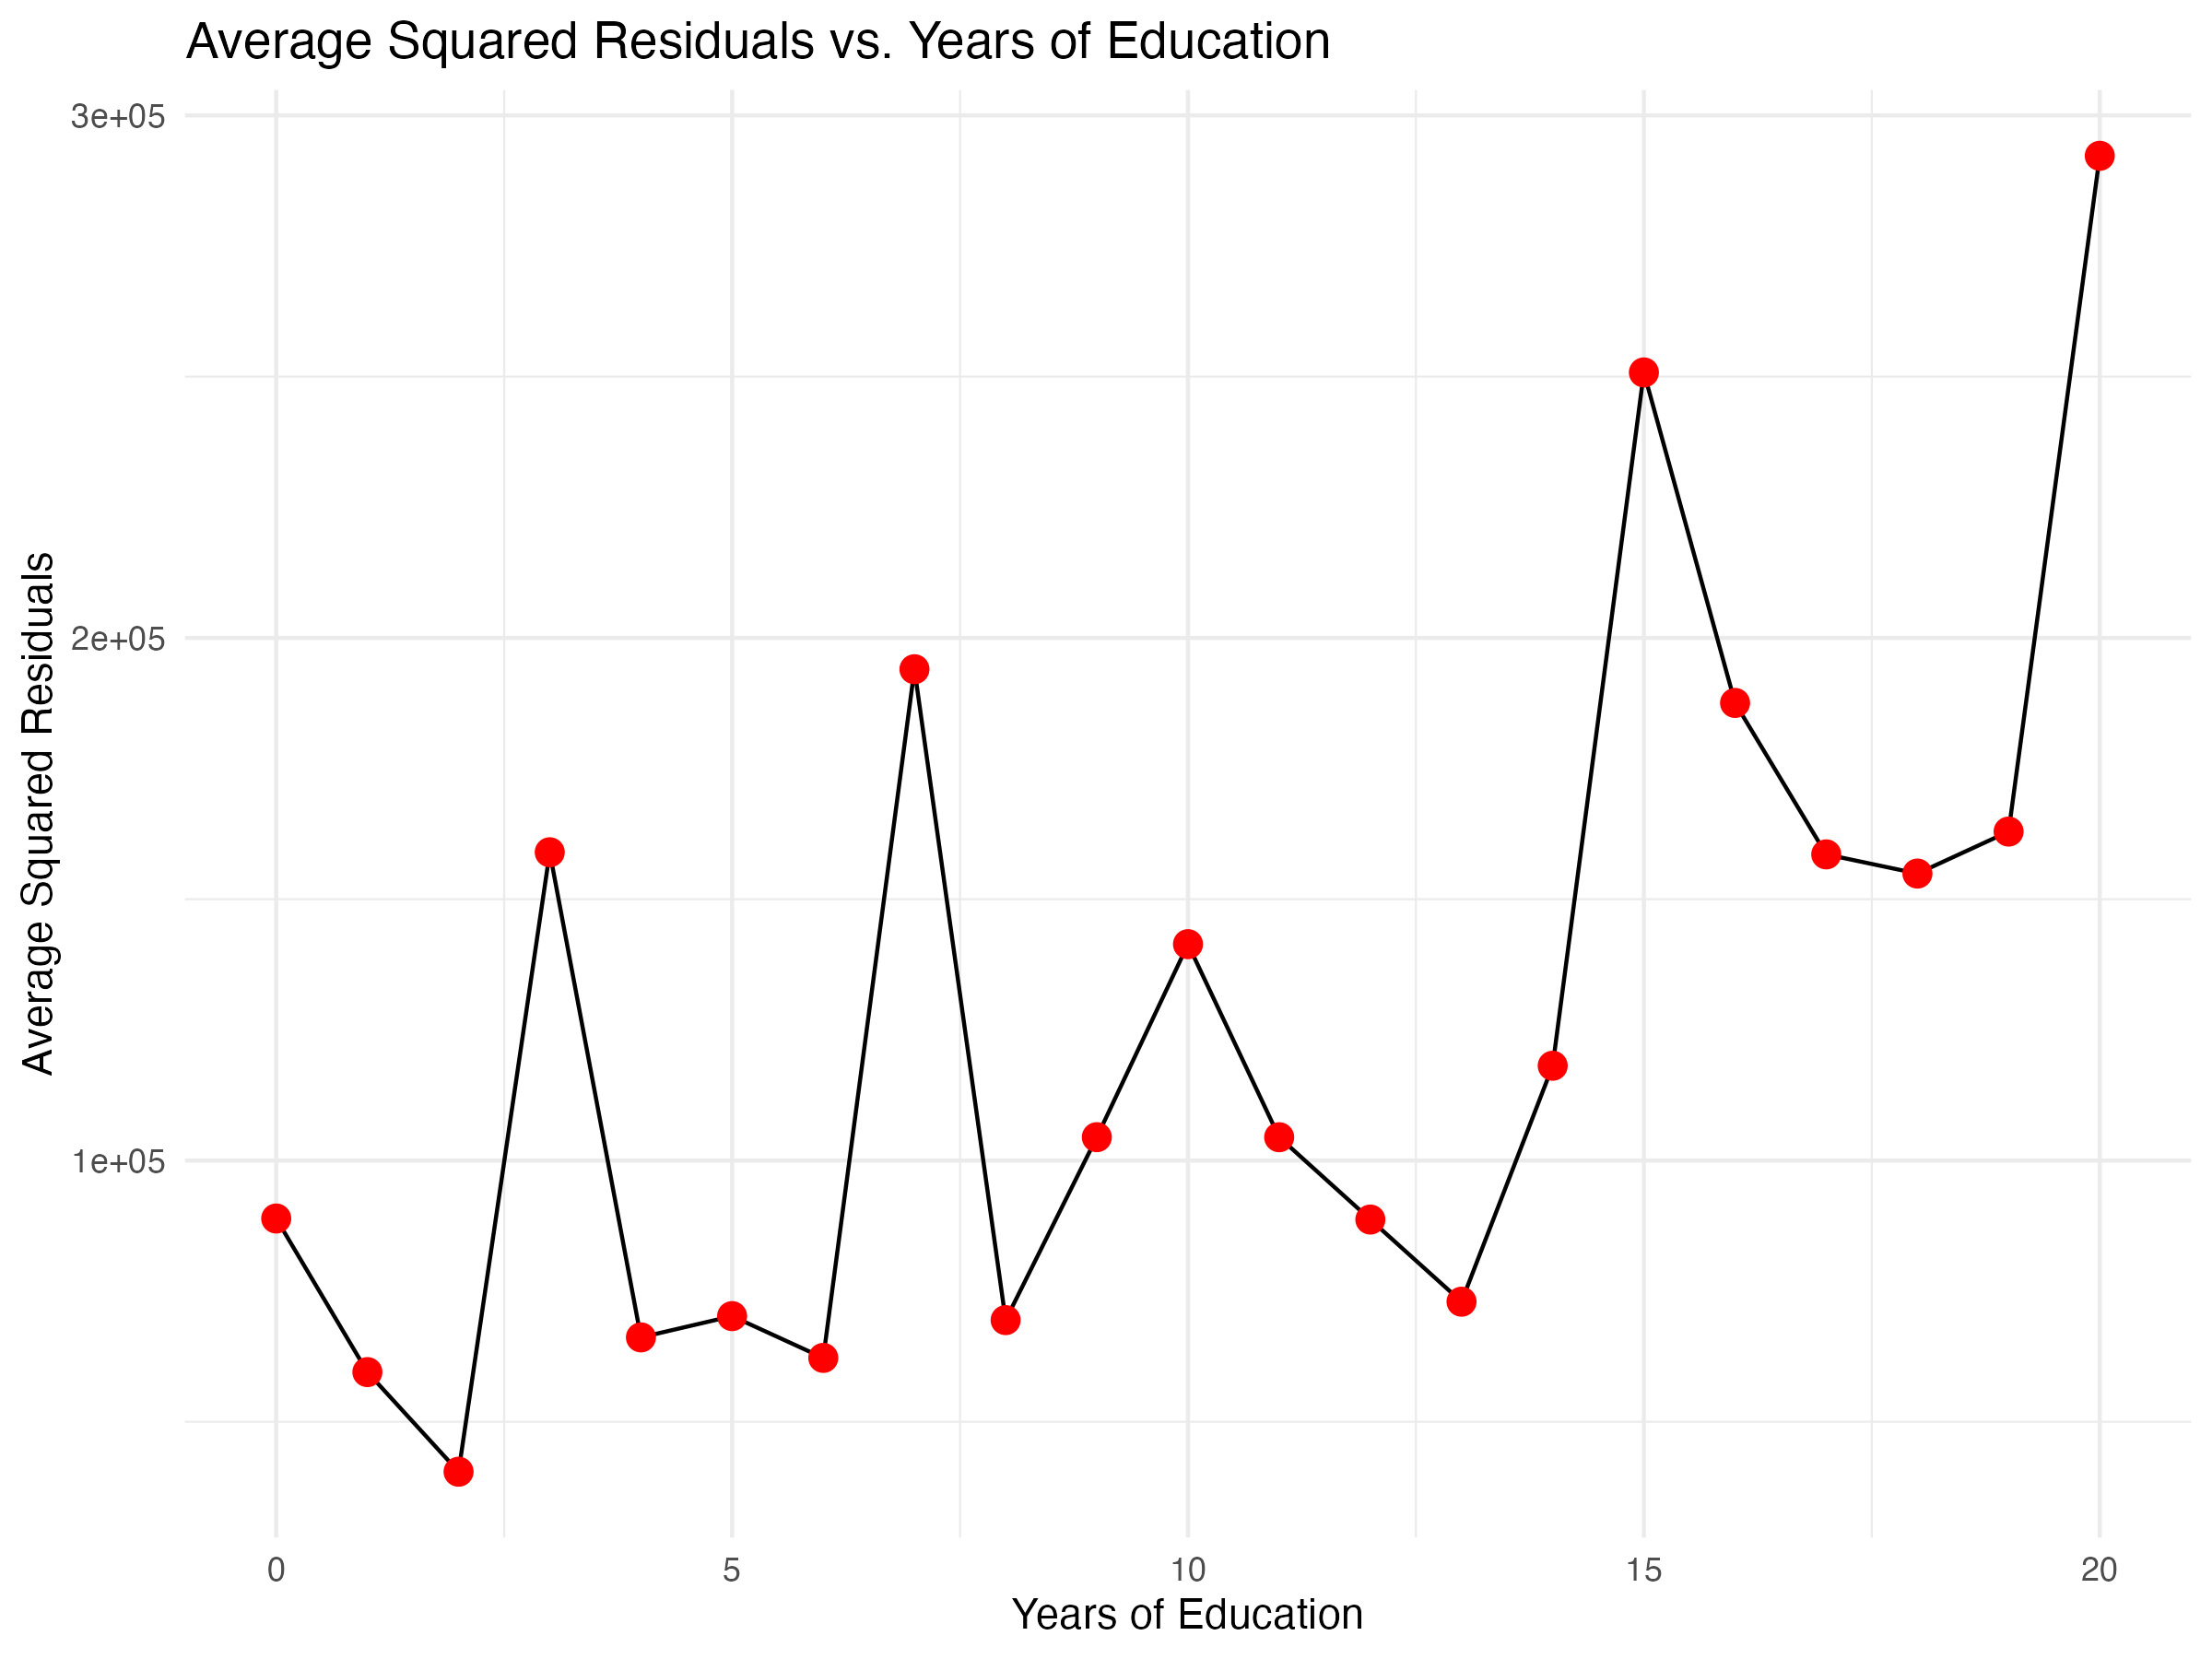
\includegraphics[width=0.8\textwidth]{output/avg_squared_residuals_vs_educ.png}
    \caption{\label{fig:avg_squared_residuals_vs_educ}Average Squared Residuals vs. Years of Education}
\end{figure}

This upward trend in the variance of residuals across education levels provides strong evidence of heteroskedasticity. The assumption of constant variance (homoskedasticity) is violated, as the error variance appears to increase with the level of education.

\subsection{Economic Interpretation}

This heteroskedasticity pattern makes economic sense. At lower education levels, wage outcomes are likely more constrained and homogeneous, leading to lower variance. However, at higher education levels, there are likely more diverse career paths and opportunities, resulting in greater wage dispersion and higher variance in the residuals.

\section{Problem 4}

As in table \ref{tab:problem_2_model} in the appendix, the homoskedastic standard errors are slightly smaller than the heteroskedastic-robust ones.
This is expected from figure \ref{fig:avg_squared_residuals_vs_educ} and the fact that mean years of education is 12.77 years.
Whereas the homoskedastic standard errors compute $\hat{\Var}({\hat\beta_1}) = \frac{\sum_{i=1}^N \hat\varepsilon_i^2}{(N-2)\sum_{i=1}^N (x_i - \bar{x})^2}$, the heteroskedastic-robust standard errors compute $\hat{\Var}({\hat\beta_1} )= \frac{\sum_{i=1}^N (x_i - \bar{x})^2 \hat\varepsilon_i^2}{\sum_{i=1}^N (x_i - \bar{x})^2 \sum_{i=1}^N (x_i - \bar{x})^2}$.
This implies that the EHW standard errors give more weights to the observations that are further away from the mean of the years of education. Since the squared residuals are much higher for higher years of education, the EHW standard errors are larger for higher years of education.


\section{Problem 5}

\subsection{Bootstrap Analysis with Small Samples (n=20)}

I conducted a bootstrap analysis using 10,000 bootstrap samples of size 20 to investigate the coverage properties of confidence intervals under both homoskedastic and heteroskedastic assumptions.

Results:
\begin{itemize}
    \item Homoskedastic model coverage: 90.83\%
    \item Heteroskedastic-robust model coverage: 90.62\%
\end{itemize}

Both models show coverage rates close to the nominal 95\% level, though slightly below. It is closer to the nominal 95\% level for the homoskedastic model, although the difference is not significantly large.
I believe this is becaues the sample size is small, so the bootstrap standard errors are not very reliable.

\section{Problem 6}

\subsection{Bootstrap Analysis with Medium Samples (n=200)}

For samples of size 200:
\begin{itemize}
    \item Homoskedastic model coverage: 91.52\%
    \item Heteroskedastic-robust model coverage: 94.70\%
\end{itemize}

\subsection{Bootstrap Analysis with Large Samples (n=2000)}

For samples of size 2000:
\begin{itemize}
    \item Homoskedastic model coverage: 91.86\%
    \item Heteroskedastic-robust model coverage: 95.32\%
\end{itemize}

\subsection{Analysis of Coverage Results}

The bootstrap results reveal important patterns:

\begin{enumerate}
    \item \textbf{Sample Size Effects}: As sample size increases from 20 to 200 to 2000, coverage rates generally improve and move closer to the nominal 95\% level.
    
    \item \textbf{Heteroskedasticity Robustness}: The heteroskedastic-robust standard errors consistently provide better coverage rates than homoskedastic standard errors, particularly as sample size increases. This confirms the presence of heteroskedasticity in the data.
    
    \item \textbf{Coverage Convergence}: The heteroskedastic-robust model achieves coverage rates very close to 95\% for larger samples (94.70\% for n=200, 95.32\% for n=2000), while the homoskedastic model remains below 95\% even for large samples.
\end{enumerate}

The analysis reveals clear evidence of heteroskedasticity in the wage-education relationship, with error variance increasing with education level. The bootstrap simulations demonstrate that heteroskedastic-robust standard errors provide better coverage properties than homoskedastic standard errors, particularly for larger samples.


\appendix
\setcounter{figure}{0}                      
\setcounter{table}{0}                      
\renewcommand\thefigure{A.\arabic{figure}} 
\renewcommand\thetable{A.\arabic{table}} 


\section{Summary Statistics}
\begin{sidewaystable}[h]
    \centering
    \tiny
    
\begin{tabular}{lrrrrrrrrrrrrrrrr}
\toprule
variable & numNA & numZeros & fracZeros & mean & sd & min & max & 10\% & 20\% & 30\% & 40\% & 50\% & 90\% & 95\% & 99\% & 99.9\%\\
\midrule
educ & 0 & 598 & 0.0018 & 12.7699 & 3.2812 & 0.0000 & 20.0000 & 9.0000 & 11.0000 & 12.0000 & 12.0000 & 12.0000 & 17.0000 & 19.0000 & 20.000 & 20.0000\\
lwage & 0 & 3 & 0.0000 & 5.8999 & 0.6788 & -2.3418 & 10.5321 & 5.2343 & 5.5218 & 5.7243 & 5.8472 & 5.9525 & 6.5567 & 6.8004 & 7.274 & 7.9495\\
yob & 0 & 0 & 0.0000 & 34.6028 & 2.9050 & 30.0000 & 39.0000 & 30.0000 & 32.0000 & 33.0000 & 34.0000 & 35.0000 & 39.0000 & 39.0000 & 39.000 & 39.0000\\
\bottomrule
\end{tabular}

    \caption{\label{tab:summary_stats}Summary Statistics}
\end{sidewaystable}


\begin{figure}[h]
    \centering
    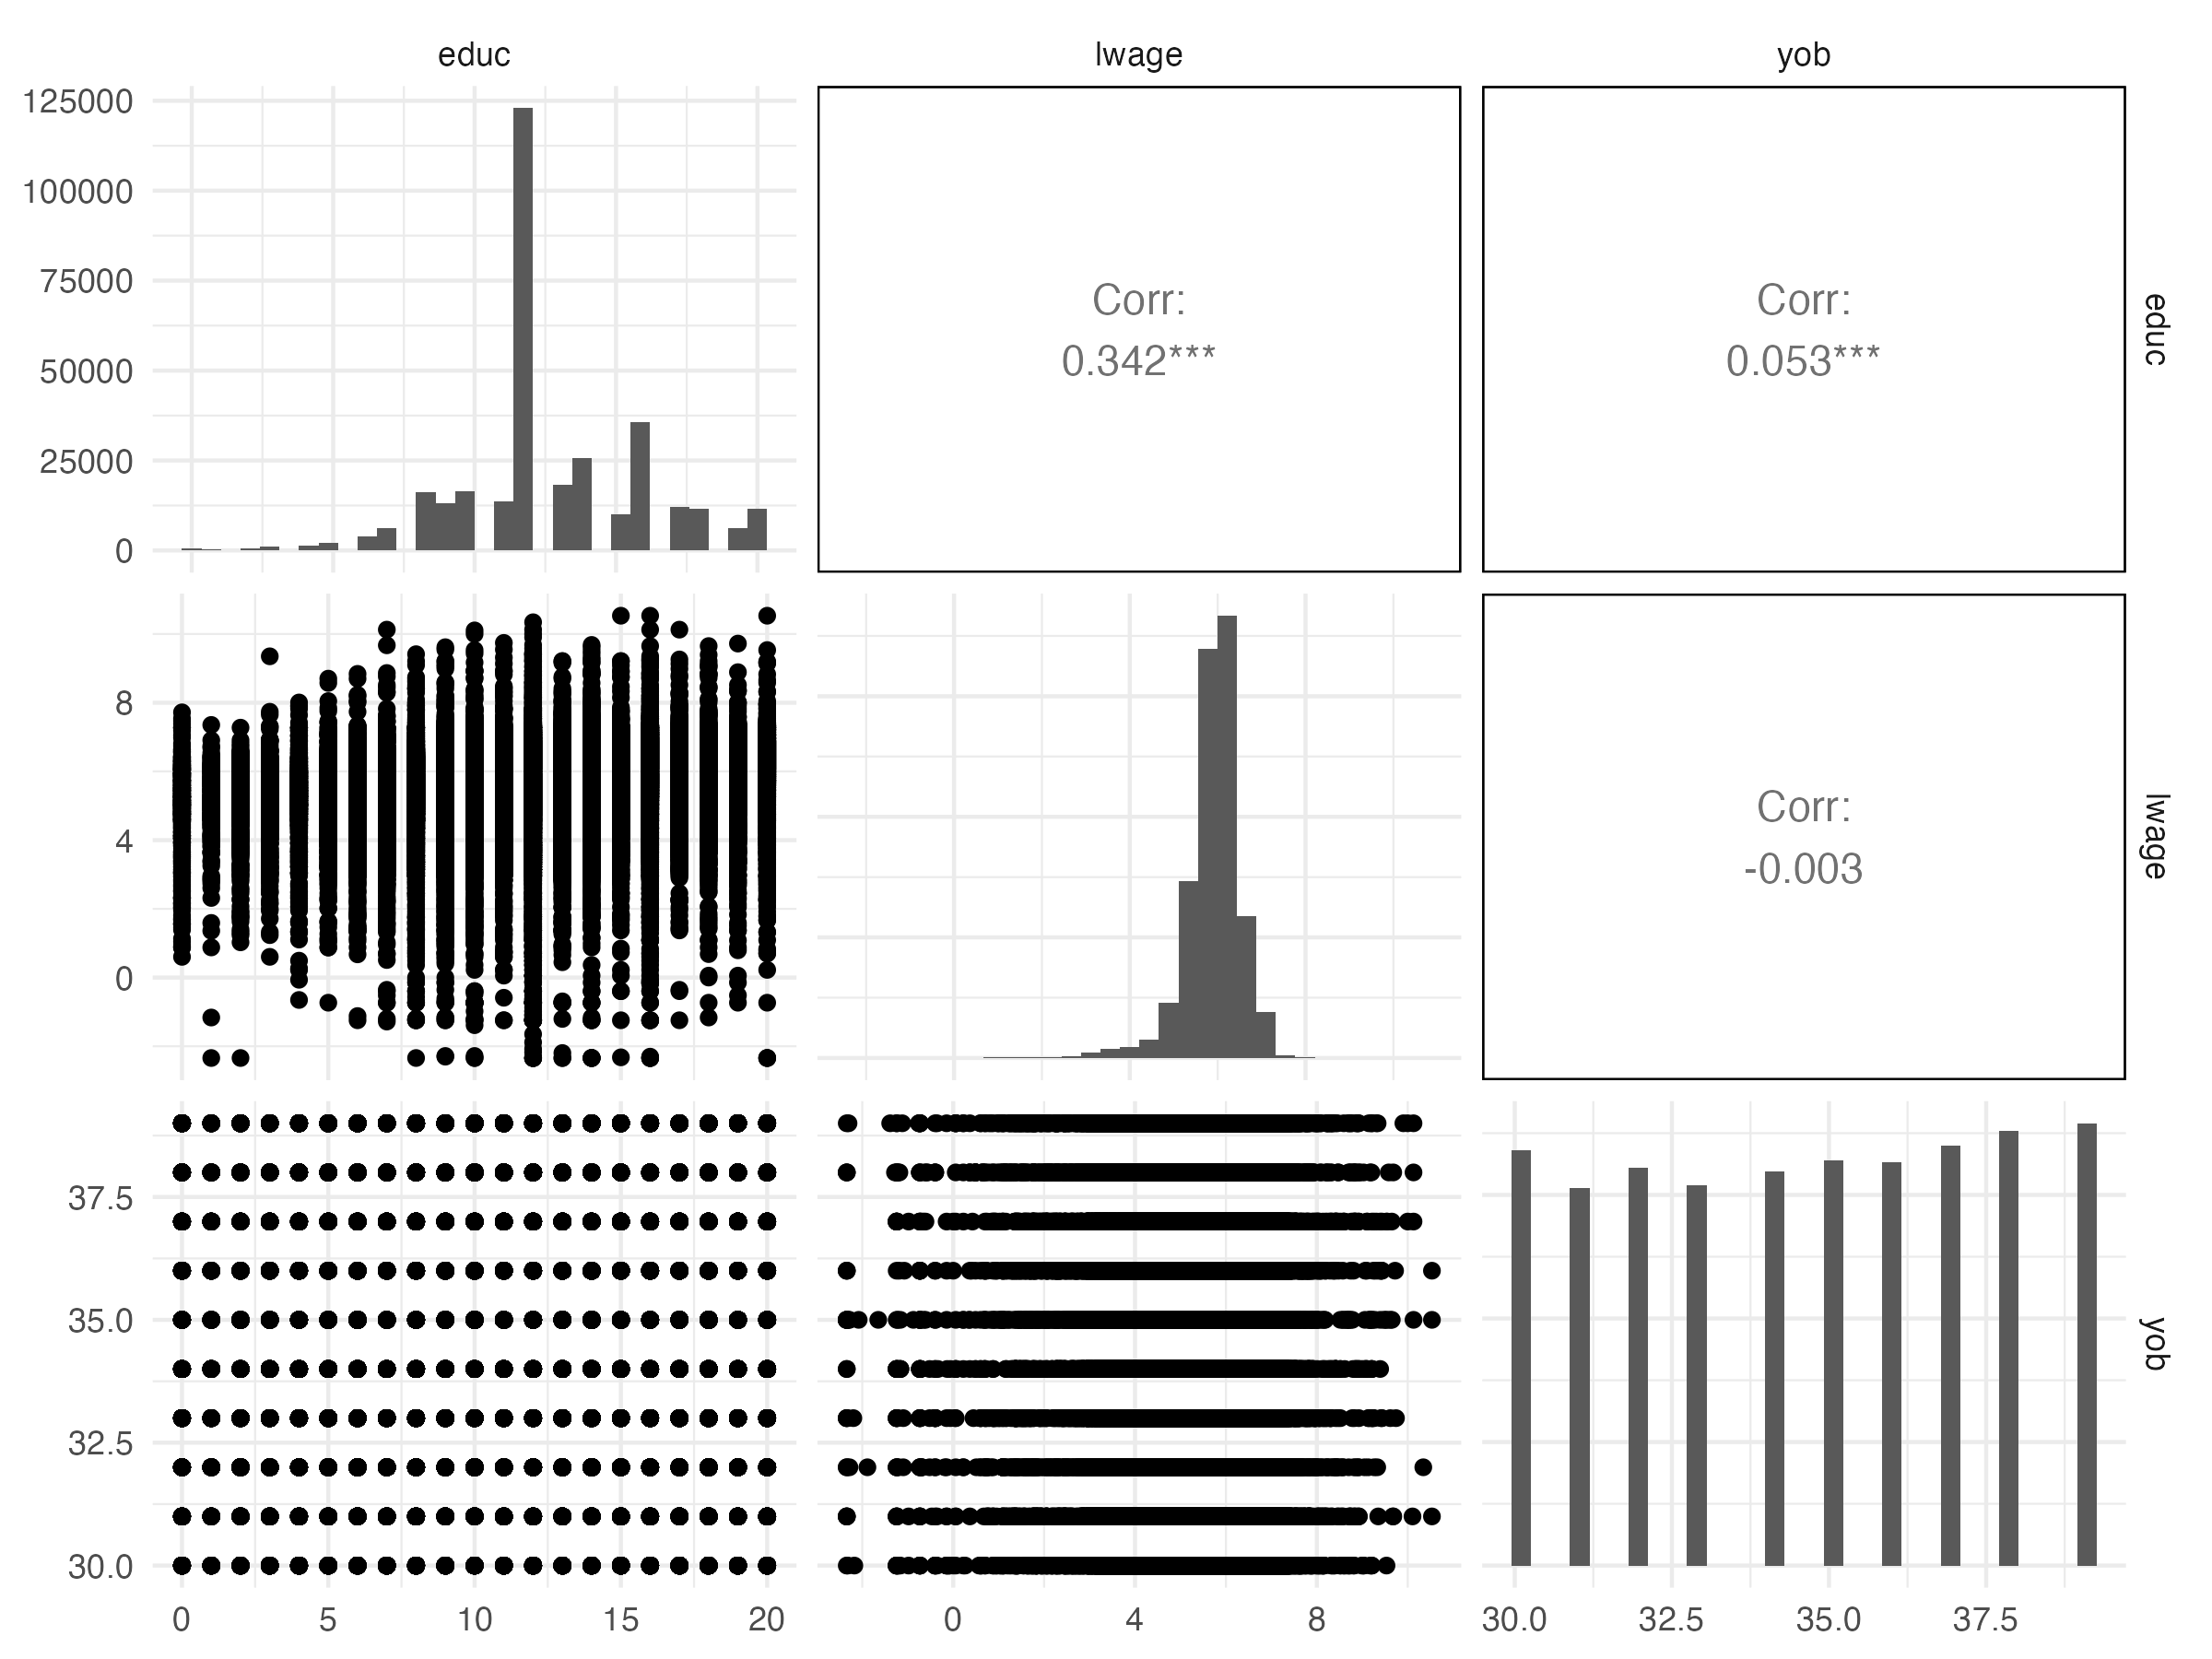
\includegraphics[width=0.8\textwidth]{output/scatterplot_matrix.png}
    \caption{\label{fig:scatterplot_matrix}Scatterplot Matrix}
\end{figure}

\section{Residual Analysis}
\begin{figure}[h]
    \begin{subfigure}{0.48\textwidth}
    \centering
    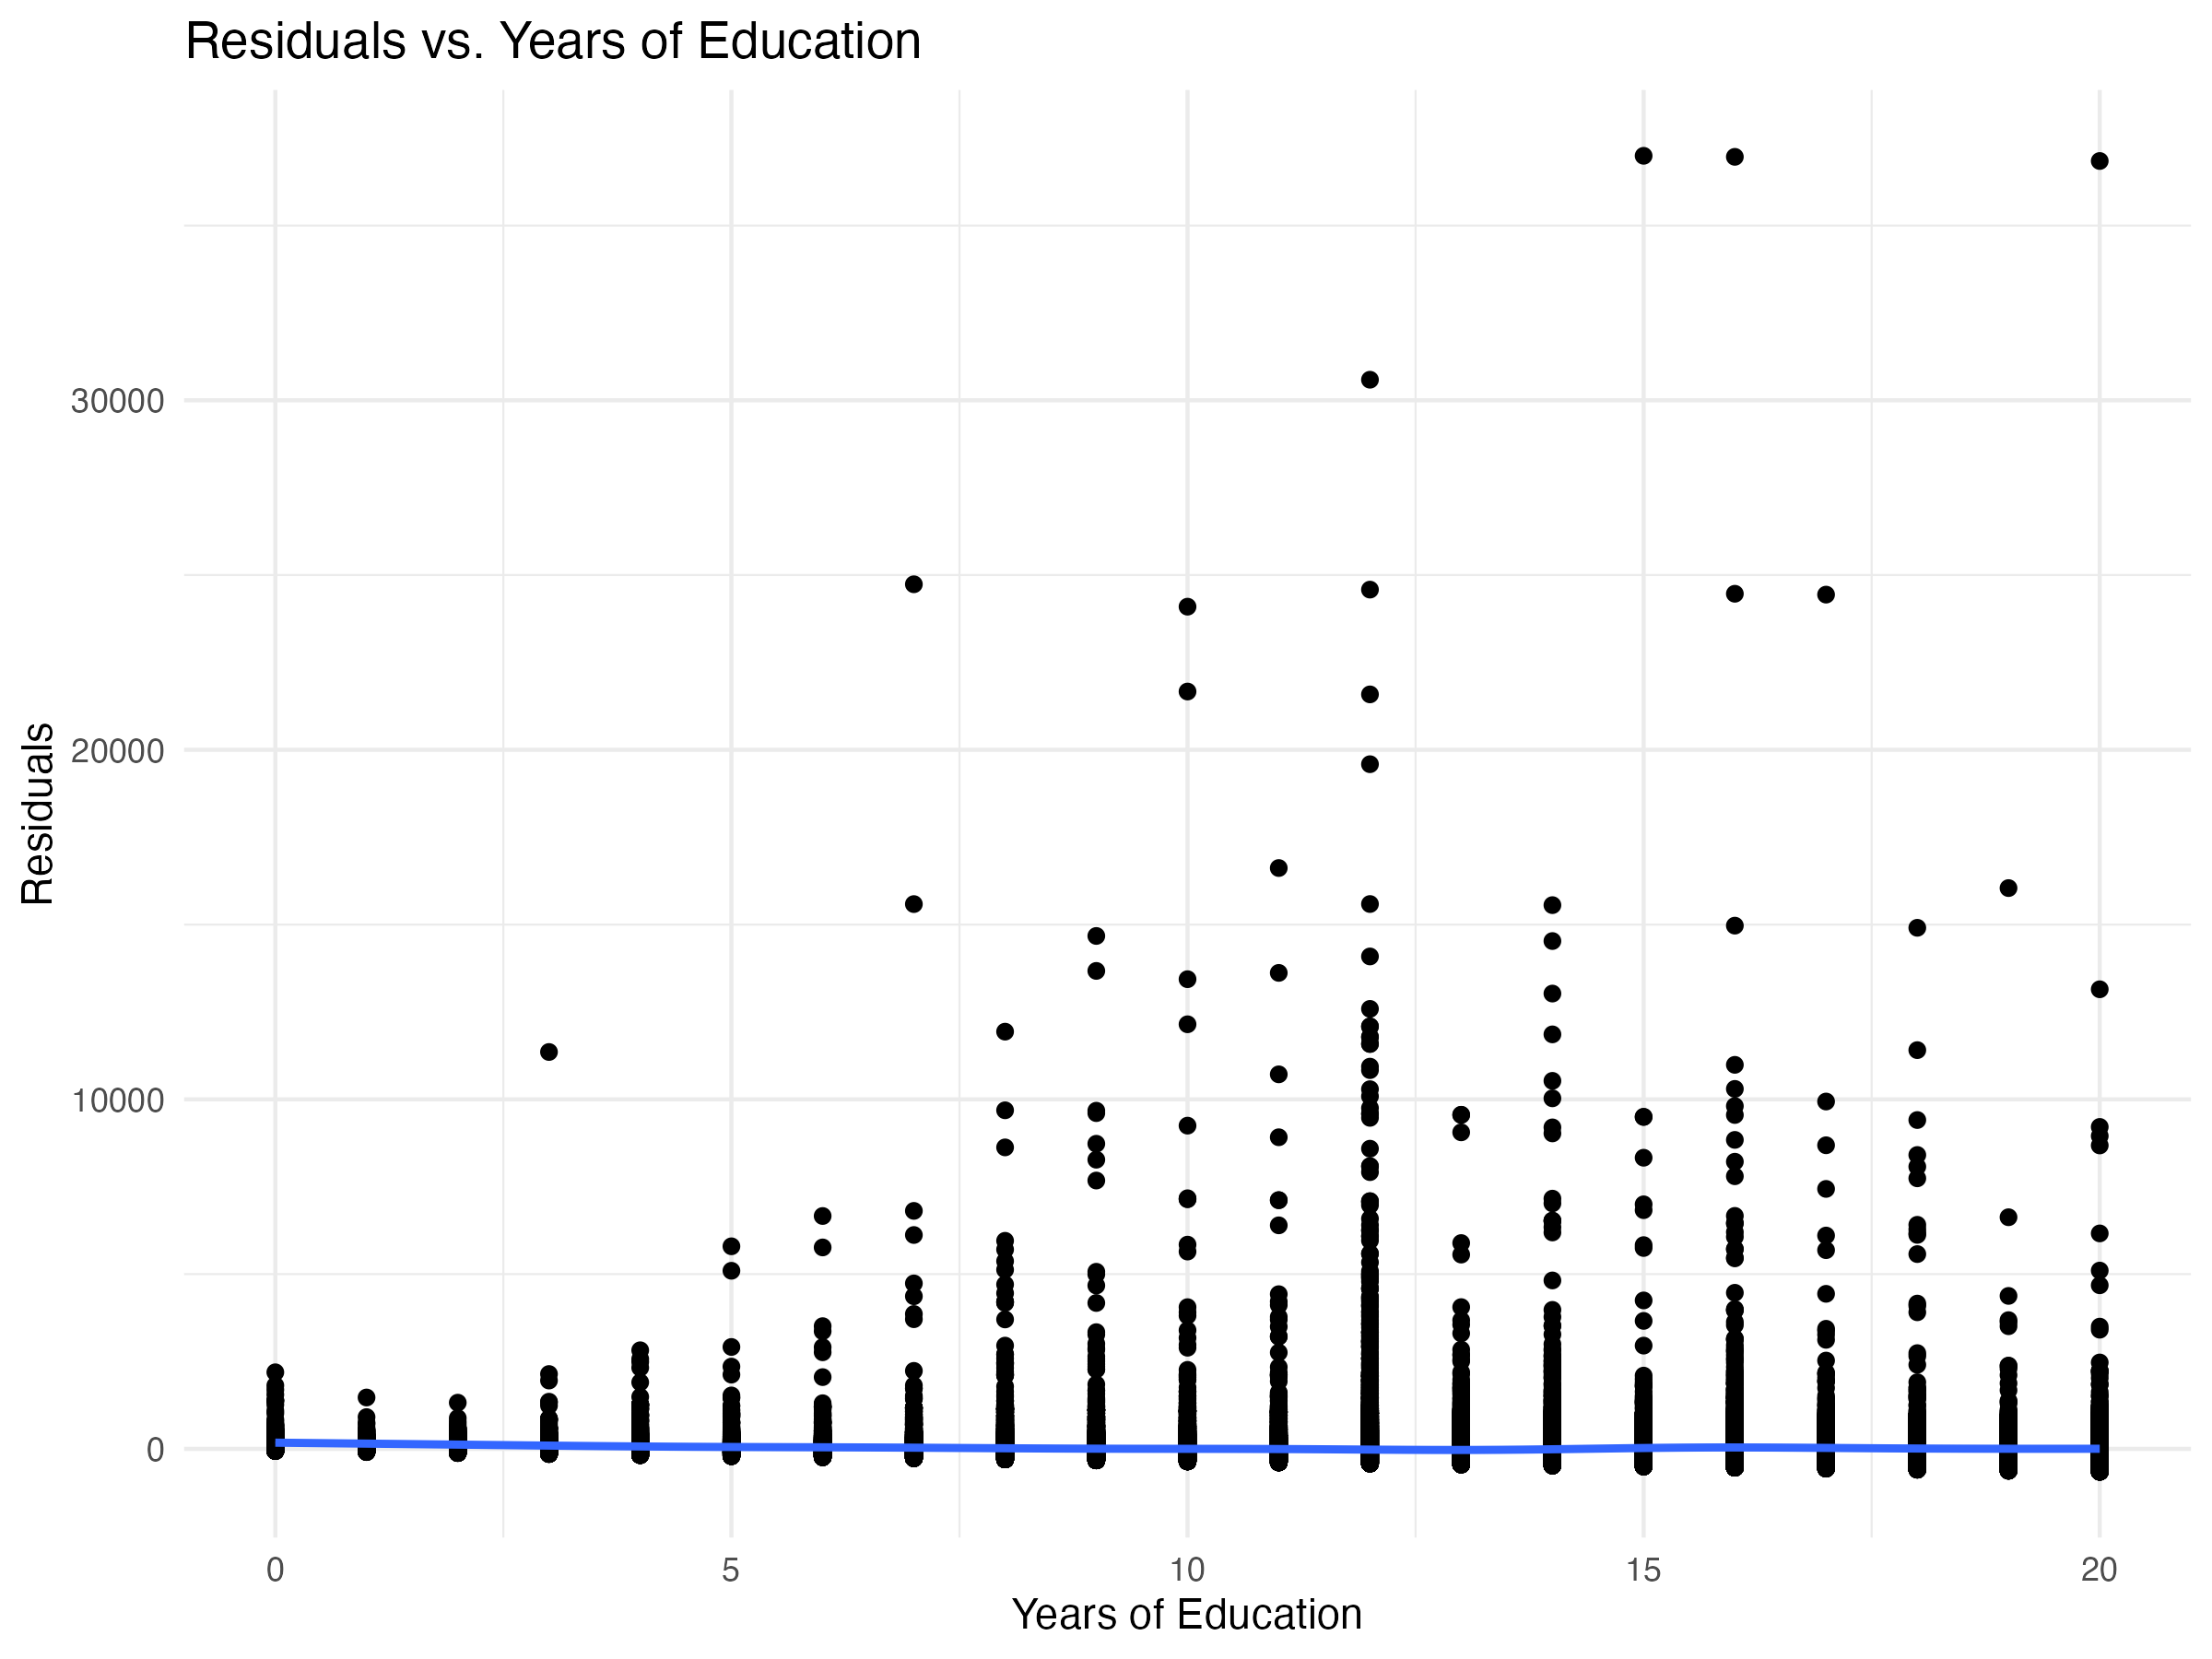
\includegraphics[width=0.8\textwidth]{output/residuals_vs_educ.png}
    \caption{\label{fig:residuals_vs_educ}Residuals vs. Years of Education}
    \end{subfigure}
    \begin{subfigure}{0.48\textwidth}
    \centering
    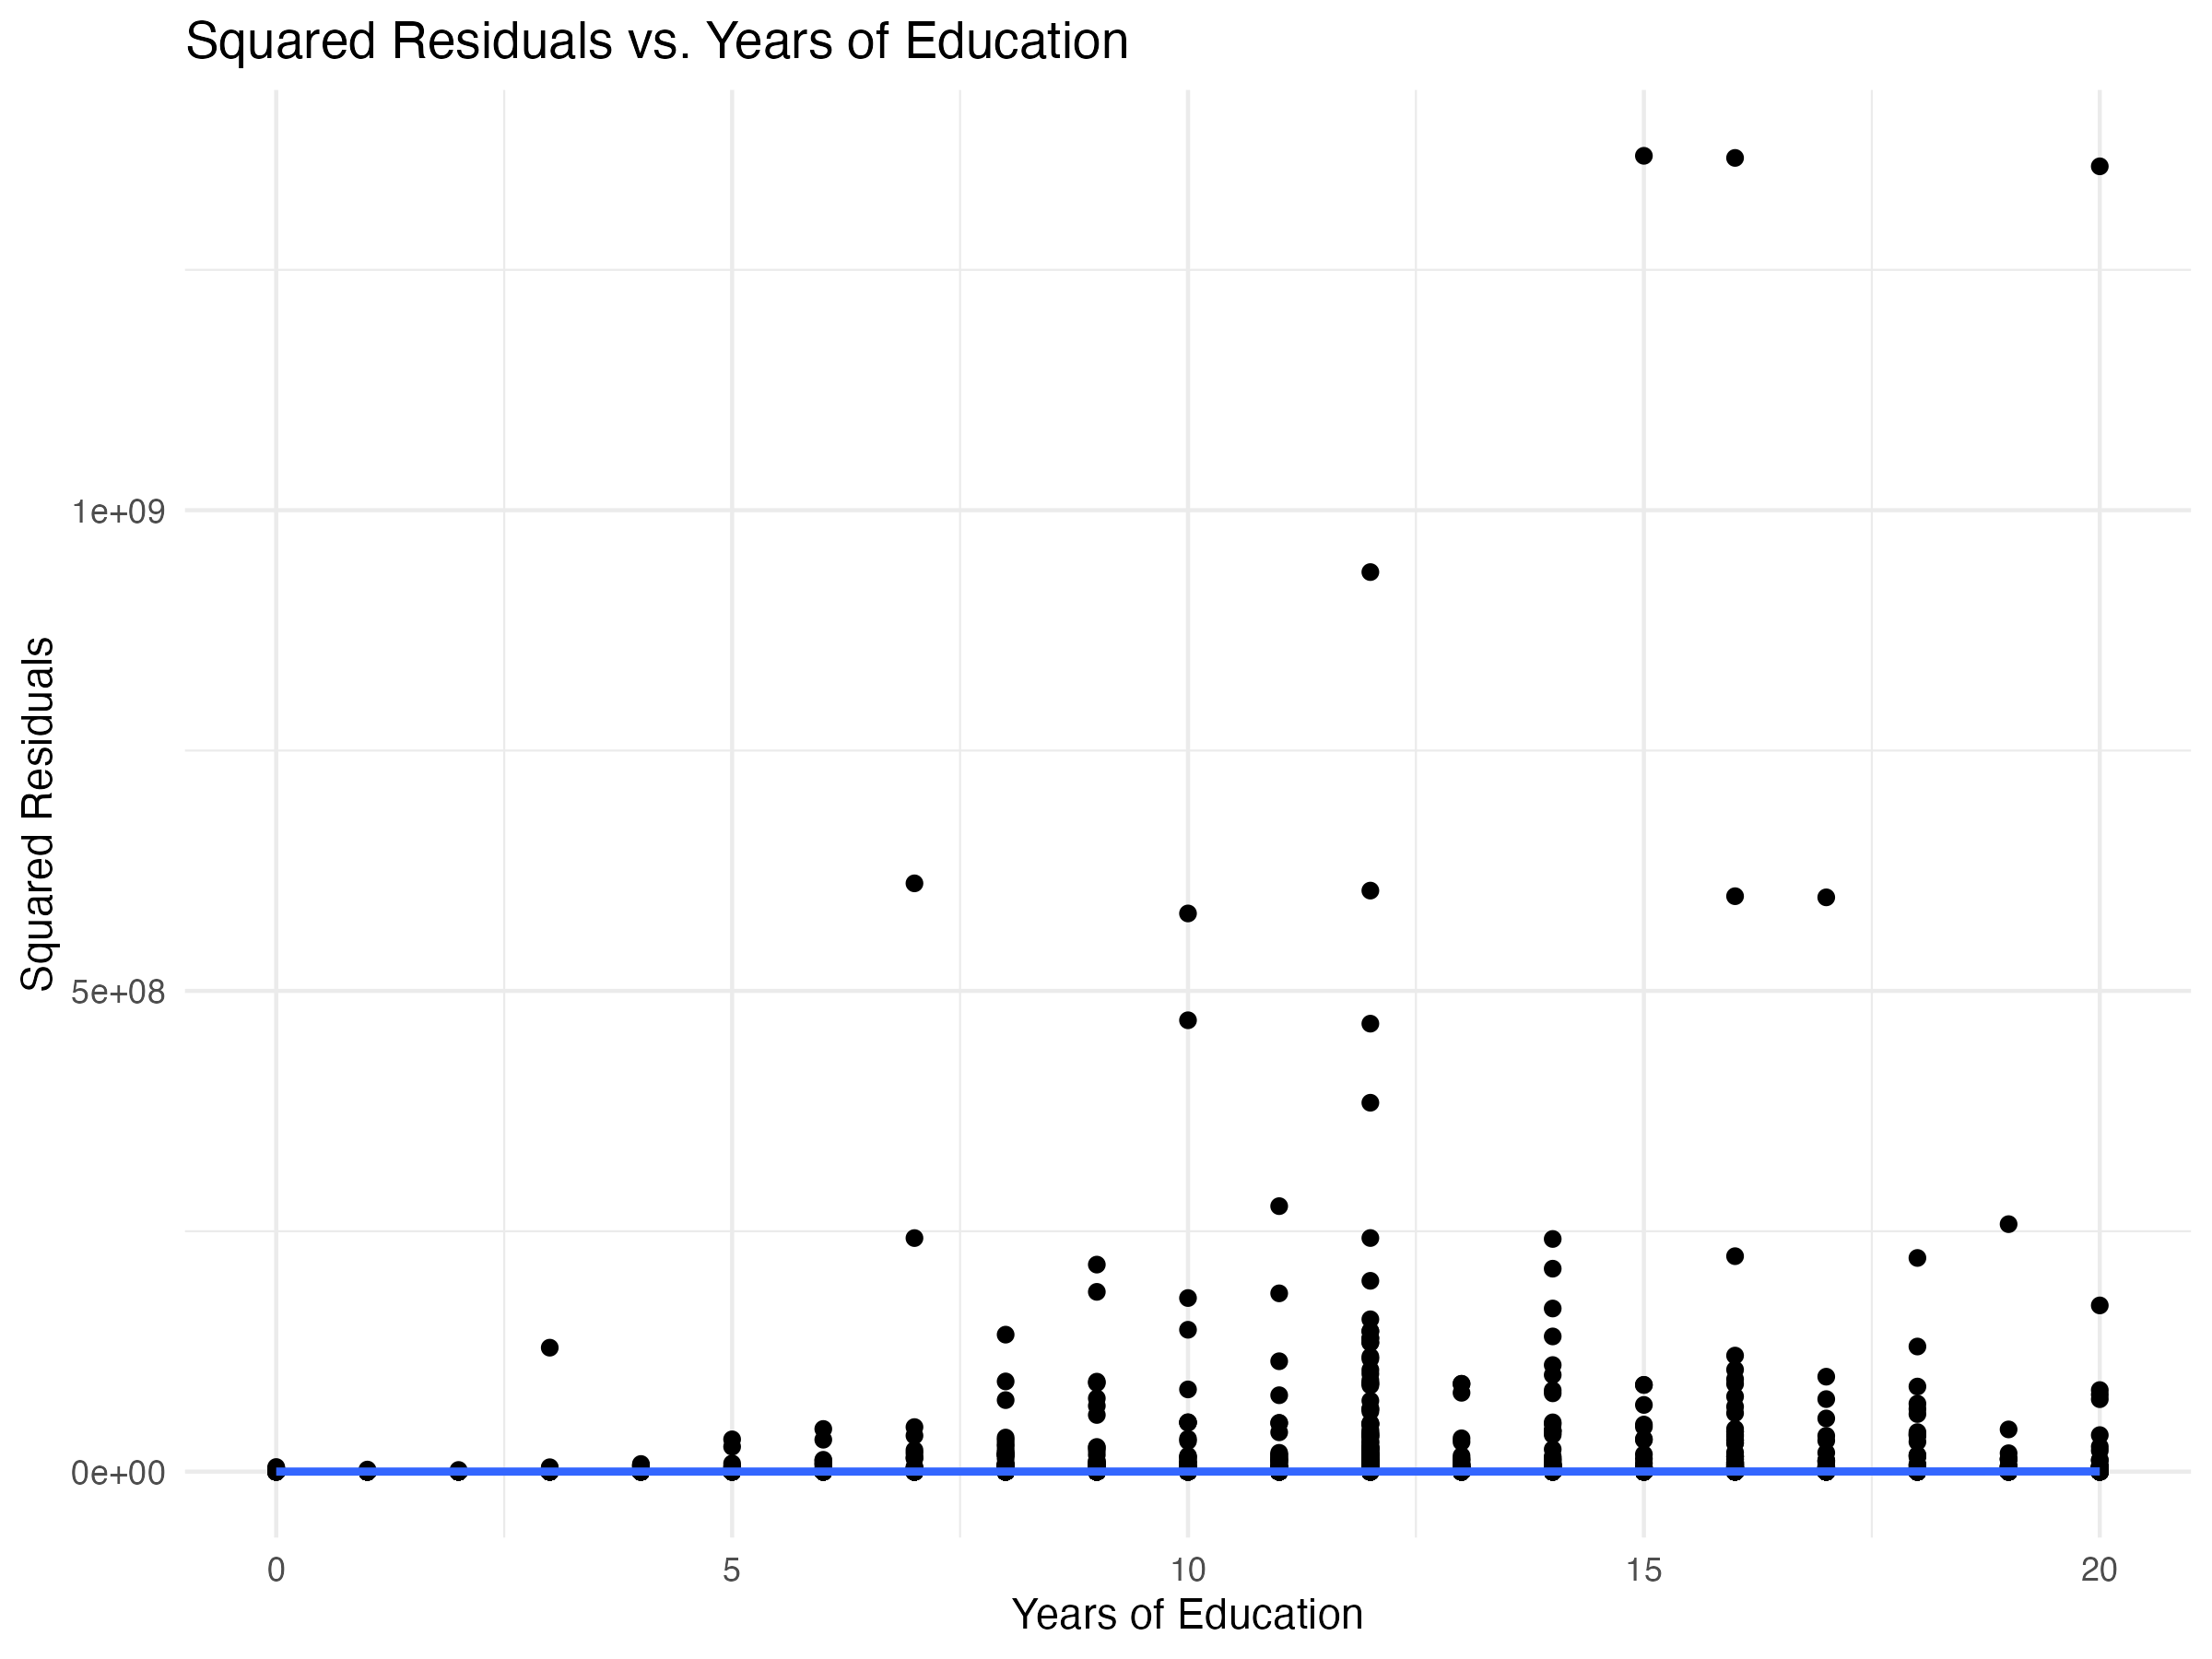
\includegraphics[width=0.8\textwidth]{output/squared_residuals_vs_educ.png}
    \caption{\label{fig:squared_residuals_vs_educ}Squared Residuals vs. Years of Education}
    \end{subfigure}
    \caption{\label{fig:residual_analysis}Residual Analysis}
\end{figure}

\end{document}